\documentclass{article}
\usepackage[a4paper, total={6in,9in}]{geometry}
\usepackage{fancyhdr}
\usepackage{graphicx}
\begin{document}
\pagestyle{fancy}
\fancyhead[L]{CS1010 -- Intro to Information Technology}
\fancyhead[R]{HW 2}
\section{Multiple Choice (5Pts)}
\begin{enumerate}
    \item Which layer in the internet protocol suite is responsible for maintaining information:
    \begin{enumerate}
        \item The Data layer
        \item The Link layer
        \item The Application layer
        \item The Transport Layer
    \end{enumerate}
    \item HTTP is
    \begin{enumerate}
        \item a set of rules for communication on the World Wide Web
        \item a language for displaying web addresses
        \item a location for something on the internet
        \item the laboratory where the World Wide Web started
    \end{enumerate}
    \item Which cloud service could I use to provide email for my company:
    \begin{enumerate}
        \item Infrastructure as a Service
        \item Software as a Service
        \item Platform as a Service
        \item all of the above
    \end{enumerate}
    \item Which is not a type of machine learning model:
    \begin{enumerate}
        \item Decision Tree
        \item Recurrent Neural network
        \item Confluence Neural network
        \item Transformer
    \end{enumerate} 
    \item The component of the computer responsible for providing power to components is the:
    \begin{enumerate}
        \item power supply
        \item power board
        \item current supply
        \item capacitor
    \end{enumerate} 
\end{enumerate}

\newpage
\section{Show Your Work}
\subsection*{Problem 1 (5 Pts)}
Below is a network to predict whether or not I should leave my house. If the output is greater than 0, I will, otherwise I won't. The inputs are the temperature (in Fahrenheit) and how cute my cat is looking (on a scale of 1 to 10). Currently, it is $10^{\circ}$F, but my cat has decided to sing the song of his people, so he's a 2 on the cute scale. Using the network and this input, calculate the value for each neuron and tell me if I should go outside:

\begin{figure}[h]
    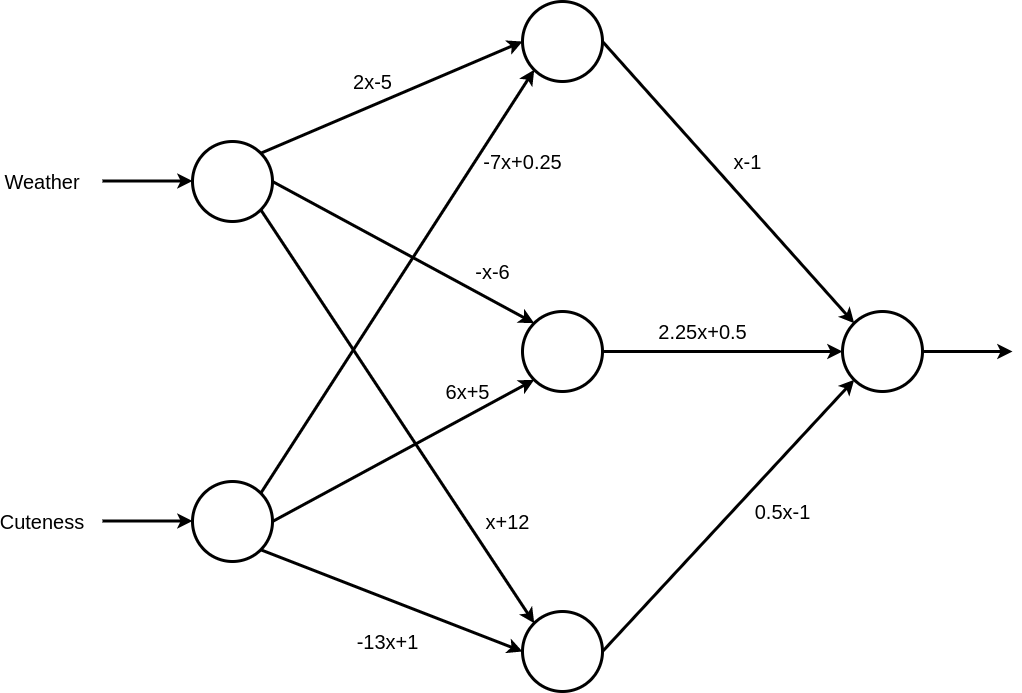
\includegraphics[width=\linewidth]{network.png}
    \label{fig:1}
\end{figure}
\newpage

\section{Short Answer}
\subsection*{Question 1 (4 Pts)}
Describe the benefits of both Wired vs Wireless internet connections:
\\[3.5in]
% \newpage
% \subsection*{Question 2 (2.5 Pts)}
% Explain the difference between Storage and Memory in computers:

\subsection*{Question 2 (4 Pts)}
Explain two benefits of using cloud computing:

\newpage

\subsection*{Question 3 (2 Pts)}
What do we mean when we say a neural network is "learning"?

\end{document}